\begin{center}
    {\LARGE \textbf{2024有机化学与分析化学}} \\[2ex]
    {\large 时量180分钟 \quad 满分150分}
\end{center}

\vspace{0.5cm}
\noindent\textbf{注意事项:}
\begin{enumerate}[label=\arabic*., parsep=0pt, itemsep=0pt]
    \item 答题前,考生先将自己的姓名、学号、考场号、座位号填写在答题卡上,将条形码准确粘贴在考生信息条形码粘贴区。
    \item 考试结束后,将本试卷与答题纸一并收回。
    \item 回答各个问题时,将答案写在答题纸上,写在本试卷上无效。
\end{enumerate}

\vspace{1cm}
\begin{center}
    {\Large \textbf{有机化学部分(共100分)}}
\end{center}

\vspace{0.5cm}
\noindent\textbf{一、选择题（15 pts.）}

\begin{enumerate}[label=\arabic*., itemsep=1.5ex]
    \item 下列共振式中贡献最大的是
    
    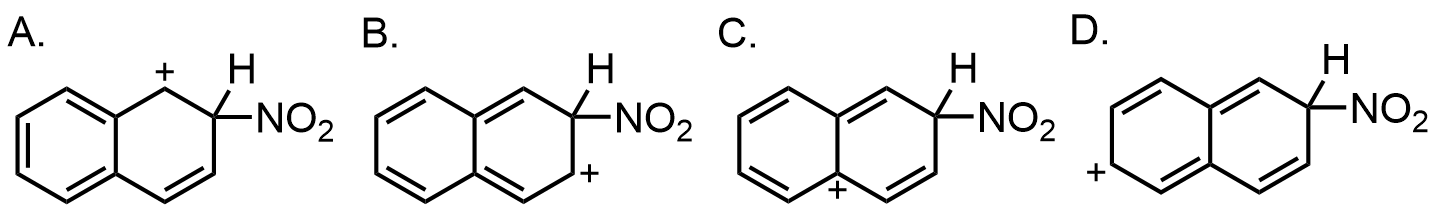
\includegraphics[scale=0.38, valign=c]{./Figure/2024/2024_4_1.png}
    \item 己二酸二乙酯在二甲苯、钠存在下生成
    
    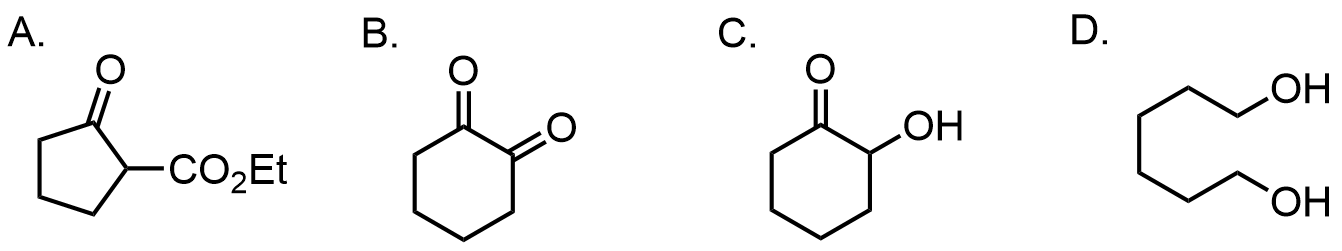
\includegraphics[scale=0.38, valign=c]{./Figure/2024/2024_4_2.png}
    \item 下列化合物亲核加成活性最高的是
    
    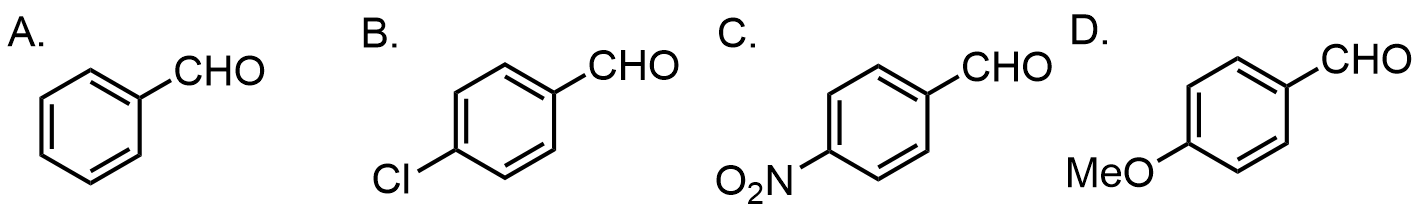
\includegraphics[scale=0.38, valign=c]{./Figure/2024/2024_4_3.png}
    \item 浓硫酸能除去苯中少量噻吩的原因是
    \begin{tasks}(1)
        \task 苯与浓硫酸互溶
        \task 噻吩与浓硫酸互溶
        \task 噻吩与浓硫酸发生亲电反应活性更高
        \task 苯与浓硫酸发生亲电反应活性更高
    \end{tasks}
    \item 将下列化合物的碱性进行排序
    
    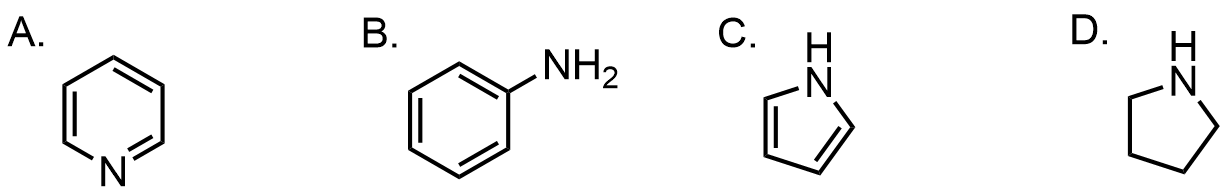
\includegraphics[scale=0.38, valign=c]{./Figure/2024/2024_4_5.png}
    \item 判断下列化合物的构型

    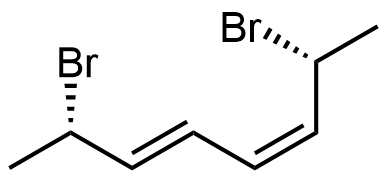
\includegraphics[scale=0.38, valign=c]{./Figure/2024/2024_4_6.png}
    \begin{tasks}(4)
        \task 2S,3E,5Z,7R
        \task 2R,3E,5S,7Z
        \task 2S,3Z,5R,7E
        \task 2R,3Z,5E,7S
    \end{tasks}
    \item 下列化合物不是内消旋体的是
    
    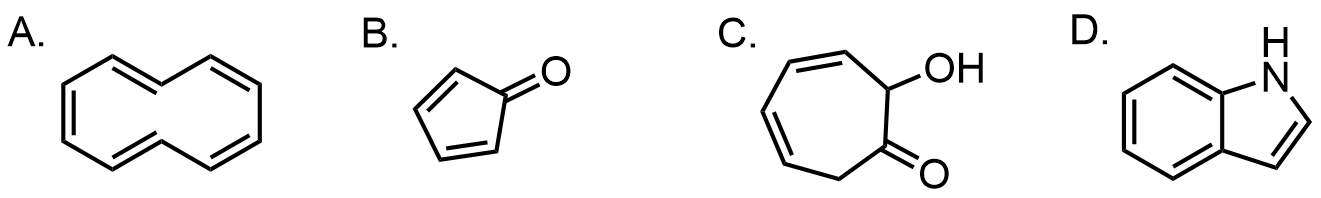
\includegraphics[scale=0.38, valign=c]{./Figure/2021/2021_4_7.png} 
    \item 给出如下反应的可能反应条件

    
\includegraphics[scale=0.38, valign=c]{./Figure/2024/2024_4_8.png}
    \begin{tasks}(2)
        \task \ce{LiAlH4}
        \task \ce{H2}/\ce{Pd-C}
        \task \ce{H2}/\ce{Pd}/\ce{BaSO4},\ce{S},Quinoline
        \task \ce{Na}/\ce{EtOH}
    \end{tasks}
    \item 不能与HCN反应的化合物是
    \begin{tasks}(4)
        \task 环戊酮
        \task 苯乙酮
        \task 苯甲醛
        \task 2-丁酮
    \end{tasks}
    \item 下列化合物碱性最强的是
    \begin{tasks}(4)
        \task \ce{CH3ONa}
        \task \ce{CH3SH}
        \task \ce{(CH3)3CONa}
        \task \ce{(CH3)2CHONa}
    \end{tasks}
    \item 顺-1-甲基-4-叔丁基最稳定的构象是
    
    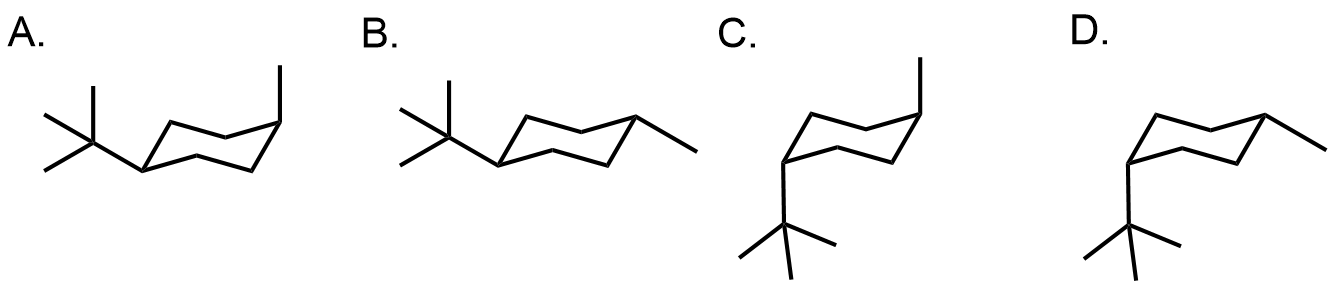
\includegraphics[scale=0.38, valign=c]{./Figure/2024/2024_4_10.png}
    \item (S)-苯基仲丁基酮在碱中长时间放置会
    \begin{tasks}(4)
        \task 构型保持
        \task 外消旋化
        \task 构型翻转
        \task 部分消旋
    \end{tasks}
    \item 3，4-二溴代吡啶与等摩尔甲醇钠反应生成
    
    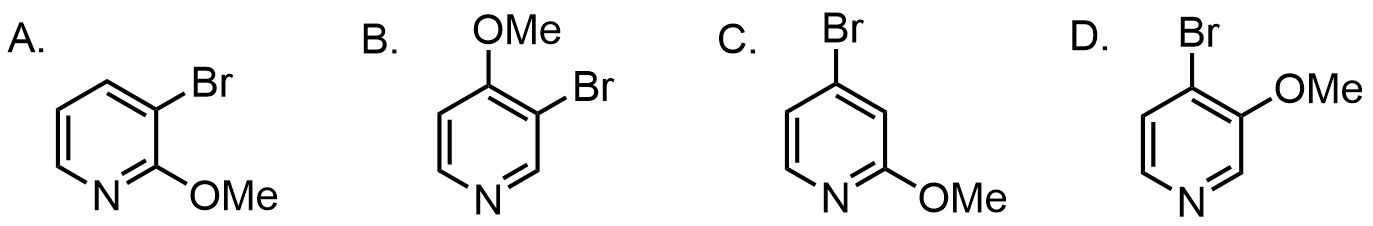
\includegraphics[scale=0.38, valign=c]{./Figure/2024/2024_4_12.png}
    \item 下列化合物中，不能发生[4+2]环加成的是
    
    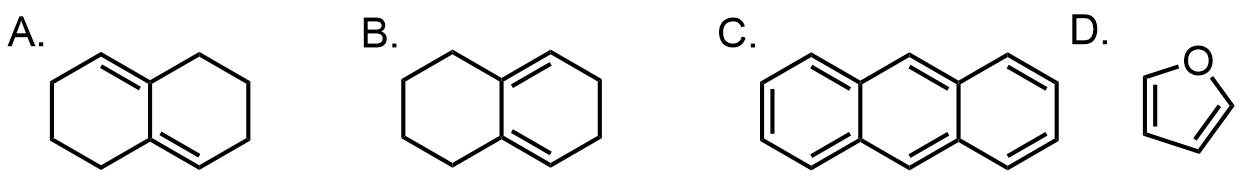
\includegraphics[scale=0.38, valign=c]{./Figure/2024/2024_4_13.png}
\end{enumerate}

\vspace{0.5cm}
\noindent\textbf{二、完成反应(30 pts.)}

\begin{enumerate}[label=\arabic*., itemsep=3ex]
    \item 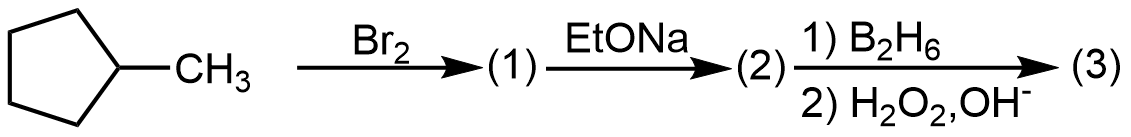
\includegraphics[scale=0.3, valign=c]{./Figure/2024/2024_1_1.png} 
    \item 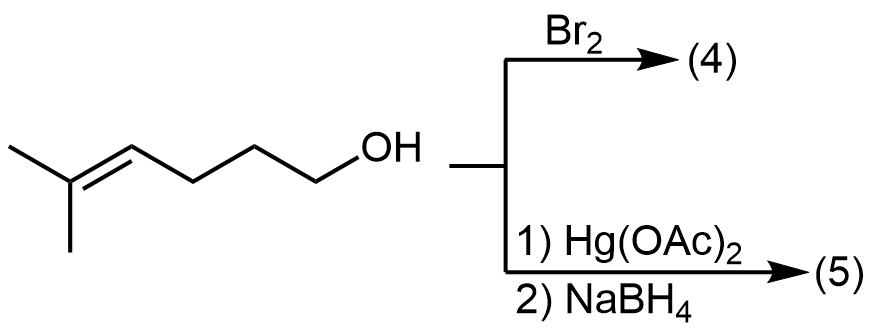
\includegraphics[scale=0.3, valign=c]{./Figure/2024/2024_1_2.png}
    \item 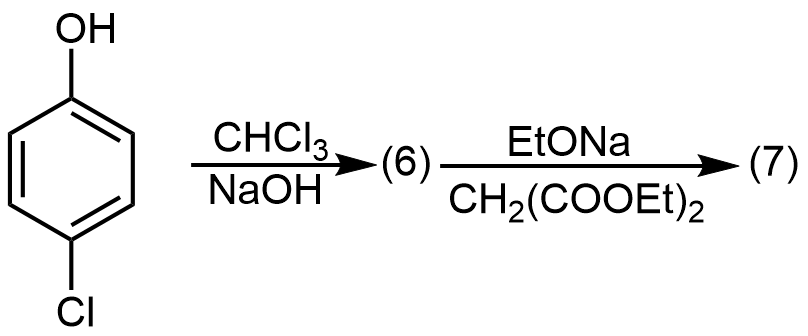
\includegraphics[scale=0.3, valign=c]{./Figure/2024/2024_1_3.png}
    \item 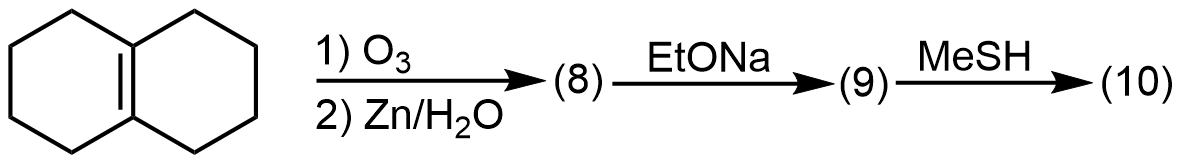
\includegraphics[scale=0.3, valign=c]{./Figure/2024/2024_1_4.png}
    \item 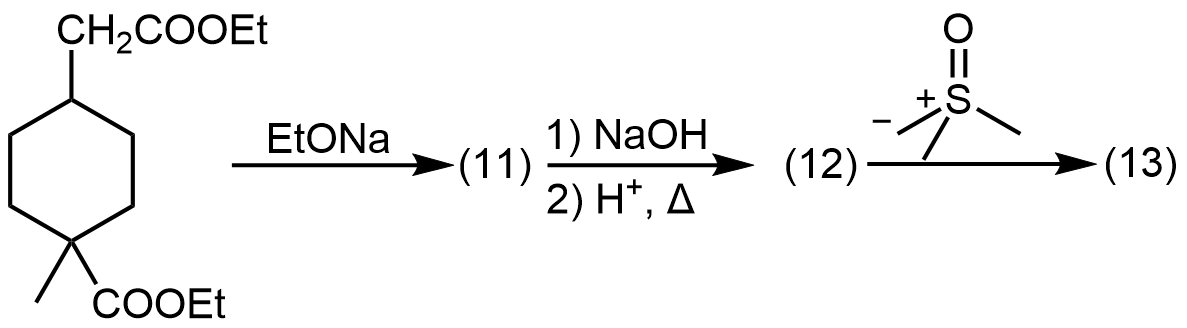
\includegraphics[scale=0.3, valign=c]{./Figure/2024/2024_1_5.png}
    \item 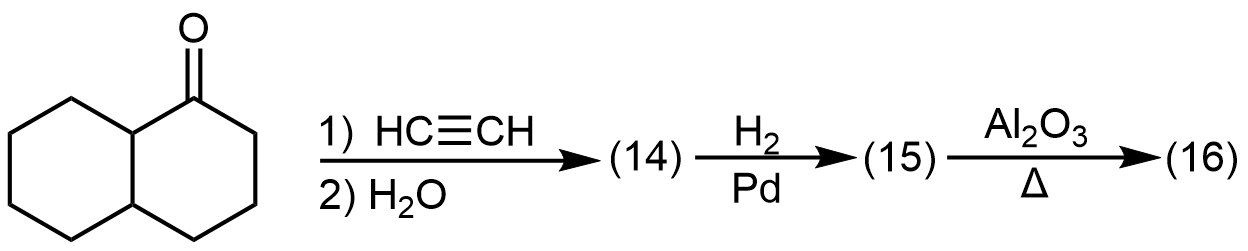
\includegraphics[scale=0.3, valign=c]{./Figure/2024/2024_1_6.png}
    \item 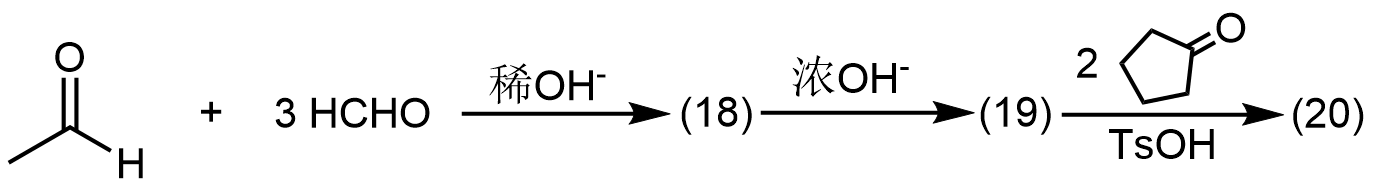
\includegraphics[scale=0.3, valign=c]{./Figure/2024/2024_1_7.png}
    \item 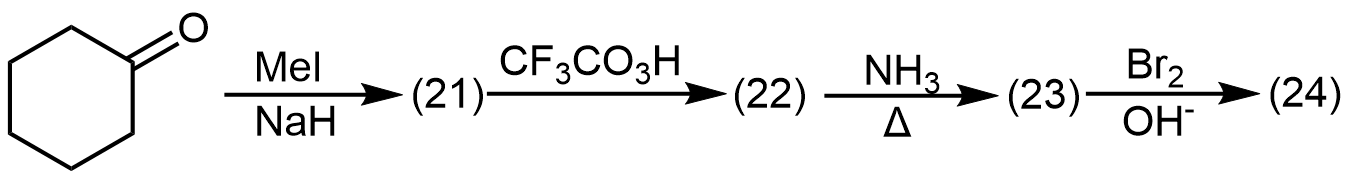
\includegraphics[scale=0.3, valign=c]{./Figure/2024/2024_1_8.png}
    \item 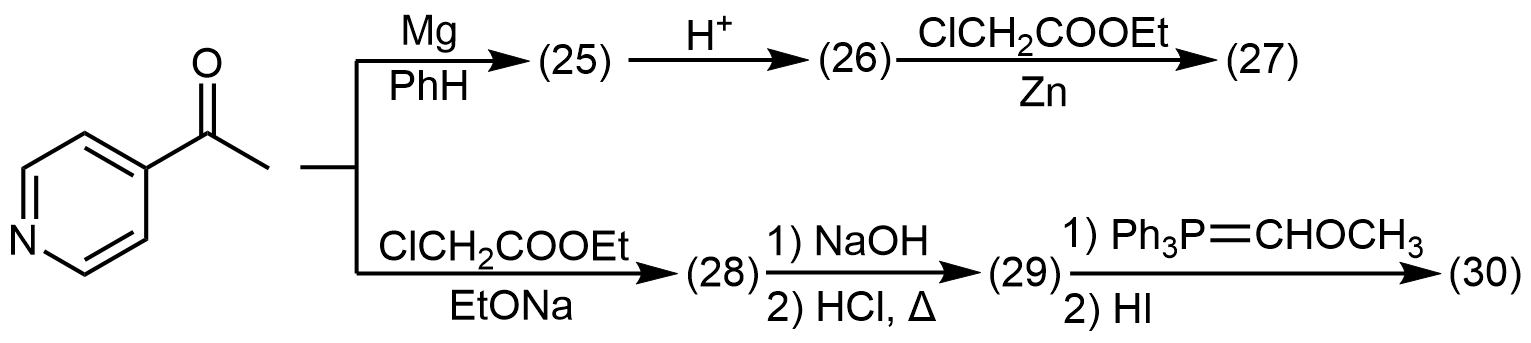
\includegraphics[scale=0.3, valign=c]{./Figure/2024/2024_1_9.png}

\end{enumerate}

\vspace{0.5cm}
\noindent\textbf{三、简答题(7 pts.)}

\begin{enumerate}[label=\arabic*., itemsep=3ex]
    \item 完成下列反应，并比较哪个反应速度快，说明原因。
    
    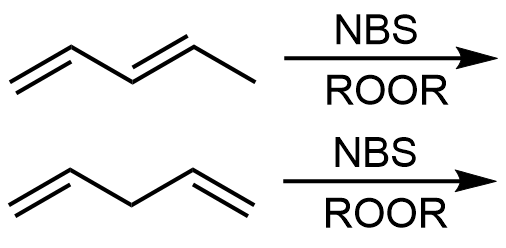
\includegraphics[scale=0.3, valign=c]{./Figure/2024/2024_5_1.png}
\end{enumerate}


\vspace{0.5cm}
\noindent\textbf{四、机理题(14 pts.)}

\begin{enumerate}[label=\arabic*., start=1, itemsep=1.5ex]
    \item 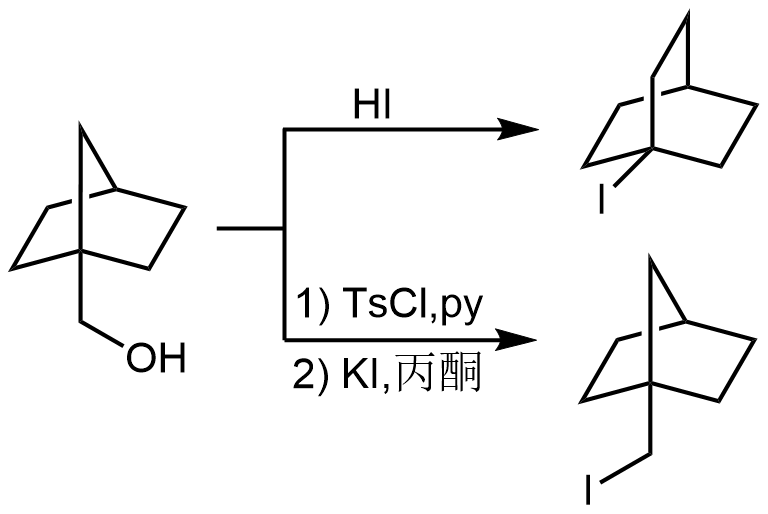
\includegraphics[scale=0.3, valign=c]{./Figure/2024/2024_2_1.png}
    \item 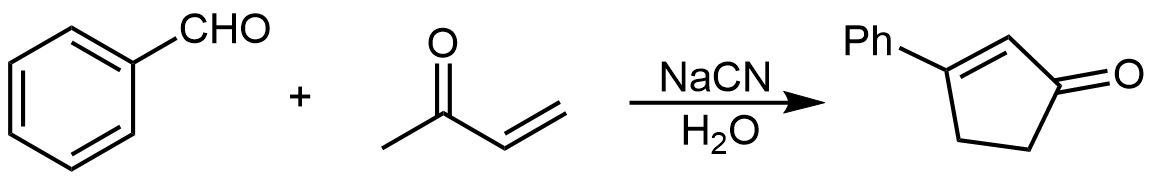
\includegraphics[scale=0.3, valign=c]{./Figure/2024/2024_2_2.png}

\end{enumerate}

\newpage

\vspace{0.5cm}
\noindent\textbf{五、合成题(35 pts.)}

\begin{enumerate}[label=\arabic*., start=1, itemsep=1.5ex]

    \begin{figure}[htbp]
        \centering
        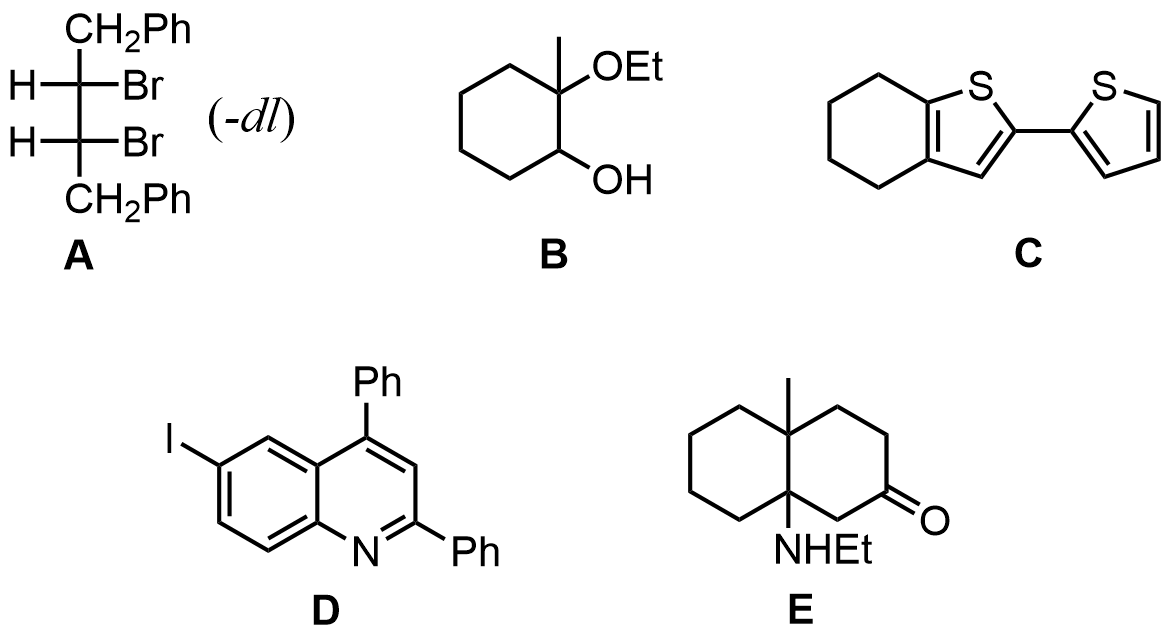
\includegraphics[scale=0.38]{./Figure/2024/2024_3.png}
    \end{figure}
    \item 用不超过两个碳的化合物和苯合成\textbf{A}
    \item 用不超过三个碳的化合物合成\textbf{B}
    \item 用环己醇、噻吩、不超过两个碳的化合物合成\textbf{C}
    \item 用不超过两个碳的化合物和苯合成\textbf{D}
    \item 用环己醇和不超过三个碳的化合物合成\textbf{E}
\end{enumerate}

\vspace{1cm}
\begin{center}
    {\Large \textbf{分析化学部分(共50分)}}
\end{center}


\noindent\textbf{六、简答题}

\begin{enumerate}
    \item 以某吸附指示剂($\text{p}K_\text{a}=7.0$)做银量法的指示剂，测定的pH应控制在什么范围？
    \item 用重铬酸钾法测定铁矿石中铁的含量，进行预处理时通常加入什么还原物质？为什么要加入$\ce{H3PO4}$？
    \item 写出下列的质子条件式：
    \begin{enumerate}
        \item 将$20\,\mathrm{mL}\ 0.10\,\mathrm{mol/L}\ \ce{NaOH}$和$10\,\mathrm{mL}\ 0.10\,\mathrm{mol/L}\ \ce{H2SO4}$的溶液混合；
        \item 将$20\,\mathrm{mL}\ 0.10\,\mathrm{mol/L}\ \ce{HCl}$溶液和$20\,\mathrm{mL}\ 0.10\,\mathrm{mol/L}\ \ce{Na2CO3}$的溶液混合。
    \end{enumerate}
    \item 对某试样进行四次分析结果如下：$29.03$、$29.08$、$28.97$、$29.24$（\%），计算平均值的置信区间。已知$t_{0.90,3}=2.35$。
    \item 向$20\,\mathrm{mL}\ 0.10\,\mathrm{mol/L}\ \ce{Ce^{4+}}$溶液中分别加入$20\,\mathrm{mL}$、$25\,\mathrm{mL}\ 0.1000\,\mathrm{mol/L}\ \ce{FeCl2}$溶液，平衡时体系的电位分别为多少？（其中$\varphi^\ominus_{\ce{Ce^{4+}/Ce^{3+}}}=1.44\,\mathrm{V},\ \varphi^\ominus_{\ce{Fe^{3+}/Fe^{2+}}}=0.68\,\mathrm{V}$）
\end{enumerate}

\vspace{1em}
\noindent\textbf{七、计算题}

\begin{enumerate}
    \item 某弱酸$\ce{HA}$总浓度为$2.0\times10^{-4}\,\mathrm{mol/L}$。于$520\,\mathrm{nm}$处，用$1\,\mathrm{cm}$比色皿测定，在不同pH值的缓冲溶液中，测得吸光度值A如下：
    \begin{center}
    \begin{tabular}{|l|ccccccc|}
    \hline
    $\text{pH}$ & $0.88$ & $1.17$ & $2.99$ & $3.41$ & $3.95$ & $4.89$ & $5.50$ \\
    \hline
    $A$ & $0.890$ & $0.890$ & $0.692$ & $0.552$ & $0.385$ & $0.260$ & $0.260$ \\
    \hline
    \end{tabular}
    \end{center}
    根据公式 $\text{p}K_\text{a} = \text{pH} + \lg\frac{A - A(\ce{A-})}{A(\ce{HA}) - A}$ ，其中$A(\ce{HA})$和$A(\ce{A-})$为酸和碱型体的吸光度，求：
    \begin{enumerate}
        \item $\ce{HA}$的$\text{p}K_\text{a}$；
        \item 用$0.02\,\mathrm{mol/L}$的$\ce{NaOH}$滴定$20.00\,\mathrm{mL}$的$0.02\,\mathrm{mol/L}\ \ce{HA}$与$0.04\,\mathrm{mol/L}\ \ce{H3BO3}$的混合溶液，滴定终点的pH为$6.5$，求化学计量点的pH及终点误差。（$\ce{H3BO3}$的$\text{p}K_\text{a}=9.24$）
    \end{enumerate}
    \item 试计算证明用沉淀掩蔽法在pH=12时用EDTA能准确滴定$\ce{Ca^{2+}, Mg^{2+}}$混合溶液中的$\ce{Ca^{2+}}$，而$\ce{Mg^{2+}}$不干扰。
    
    [已知$\ce{Ca^{2+}, Mg^{2+}}$及EDTA浓度均为$0.020\,\mathrm{mol/L}$，$\ce{Mg(OH)2}$的$\text{p}K_\text{sp}=10.7$，$\lg K_{\ce{CaY}}=10.7$，$\lg K_{\ce{MgY}}=8.7$，pH=12时$\lg\alpha_{Y(\text{H})}=0$]
    \item 求$\ce{AgCl}$沉淀在pH=8的HL溶液中的溶解度。其中HL的总浓度为$0.10\,\mathrm{mol/L}$，$K_\text{sp}(\ce{AgCl})=1.8\times10^{-10}$，$\ce{Ag+}$与$\ce{L-}$络合物的$\lg\beta_1=3.0,\ \lg\beta_2=7.0$，且$K_\text{a}(\ce{HL})=1.0\times10^{-10}$。
\end{enumerate}